\chapter{Background Estimation}
\label{ch:6}

% **************************** Define Graphics Path **************************
\ifpdf
    \graphicspath{{Chapter6/Figs/Raster/}{Chapter6/Figs/PDF/}{Chapter6/Figs/}}
\else
    \graphicspath{{Chapter6/Figs/Vector/}{Chapter6/Figs/}}
\fi

Predictions of EWK SM backgrounds are made using independent, process-specific 
control regions. These regions are orthogonal to the signal region due to the 
selection of leptons or photons - particles which are subsequently ignored such 
that the selection kinematics of each event is kept similar to the corresponding process 
observed in the signal region. For each sample, Transfer Factors (TF) are 
constructed from yields in MC, to extract a prediction in the signal 
region for a given process. This process is described at length in
section~\ref{sec:background_overview}.

Predictions made using this technique alone are considered as ``primitive'' 
predictions and are used only in analysis development and the derivation of 
background systematics. In order to determine final yields for interpretation and 
limit-setting, a fit is made across all signal and control regions, using the 
likelihood model, described later in chapter~\ref{ch:7}. The derived 
transfer factors and individual yields enter as terms in the likelihood, where 
all related systematics, potential correlations and signal contamination are
accounted for.

% Thresholds of the \alphat variable are determined such that the QCD MJ 
% contribution to the SM background is negligible. These are found using a
% data-driven method, employing sidebands in both the \mhtmet and \alphat variables, 
% described in section~\ref{sec:background_qcd}. Following the 
% application of these thresholds, any QCD contributions are considered negligible
% and are therfore not considered in the likelihood model.

%********************************** % First Section  *************************************
\section{Overview of Electroweak background prediction method}  %Section - 1.1 
\label{sec:background_overview}

Contributions from Standard Model background processes are estimated using a data-driven 
prediction technique, employing dedicated control samples. A transfer factor 
is constructed from MC samples as the ratio 
of the MC yield in the signal region, \\$N_{MC}^{signal}\big(\HT, \nj, \nb\big)$,
and the MC yield of a given control region, \\$N_{data}^{control}\big(\HT, \nj, \nb\big)$,
as a function of the analysis binning, \HT, \nj and \nb, defined as:
% 
\begin{equation}
TF = \frac{N_{MC}^{signal}\big(\HT, \nj, \nb\big)}{N_{MC}^{control}\big(\HT, \nj, \nb\big)} .
\label{eq:transfer_factor}
\end{equation}
% 
For a given \HT, \nj and \nb bin, the TF is used to extrapolate a yield in data from
the control region, $N_{data}^{control}\big(\HT, \nj, \nb\big)$
to the signal region $N_{pred}^{signal}\big(\HT, \nj, \nb\big)$, using:
% 
\begin{equation}
N_{pred}^{signal}\big(\HT, \nj, \nb\big) = N_{data}^{control}\big(\HT, \nj, \nb\big)
\times TF .
\label{eq:transfer_equation}
\end{equation}
% 
The control samples are statistically independent and each used for predicting 
specific background processes, the details of which are described in
section~\ref{sec:background_control}.

MC yields are defined by process from the following samples:
W + jets (\numw),
\ttbar + jets (\numtt), DY + jets (\numdy), $\gamma$ + jets(\numgam),
single top + jets (\numtop), WW + jets, WZ + jets and ZZ + jets (\numdibo), and
\zinv + jets (\numzinv).

% Predictions made using this technique alone are considered as ``na\"{i}ve'' 
% predictions and are used only in analysis development and the derivation of 
% background systematics. In order to determine final yields for interpretation and 
% limit-setting, a fit is made across all signal and control regions, using the 
% full likelihood model, described later in chapter~\ref{ch:7}. The derived 
% transfer factors and individual yields enter as terms in the likelihood, where 
% all related systematics, potential correlations and signal contamination are
% accounted for in the fit. 

The denominator of each transfer factor is constructed using the sum of
\textit{all} MC sample yields, for a given control region selection and
analysis category:
% 
\begin{equation}
N_{MC}^{control}\big(\HT, \nj, \nb\big) = \numw + \numtt + \numdy + \numgam + 
\numtop + \numdibo + \numzinv .
\label{eq:trans_fact_denom}
\end{equation}
% 
The numerator is constructed according to the b-tag multiplicity being 
considered. For $\nb \leq 1$, the \mj control region is used to predict 
lost-lepton background, e.g. \ttbar + jets and W + jets. All MC samples
are therefore used with the exception of \zinv:
% 
\begin{equation}
N_{MC}^{signal}\big(\HT, \nj, \nb \leq 1\big) = \numw + \numtt + \numdy + \numgam + 
\numtop + \numdibo .
\label{eq:trans_fact_num_le1b_noz}
\end{equation}
% 
The \zinv + jets component of the background is predicted using the \mmj
and \gj control samples, using only the \zinv MC yields:
% 
\begin{equation}
N_{MC}^{signal}\big(\HT, \nj, \nb \leq 1 \big) = \numzinv .
\label{eq:trans_fact_num_le1b_z}
\end{equation}
%
For $\nb \geq 2$, the \mj sample is used to produce a prediction for all 
SM processes, including \zinv, and therefore the numerator of the TF is defined as:
% 
\begin{equation}
N_{MC}^{signal}\big(\HT, \nj, \nb \geq 2 \big) = \numw + \numtt + \numdy + \numgam + 
\numtop + \numdibo + \numzinv ,
\label{eq:trans_fact_num_geq2b}
\end{equation}
% 
or equivalently:
% 
\begin{equation}
N_{MC}^{signal}\big(\HT, \nj, \nb \geq 2 \big) = N_{MC}^{signal}\big(\HT, \nj, \nb \leq 1\big) + \numzinv .
\end{equation}

The \mmj and \gj control samples are not used beyond the $\nb \leq 1$ categories
due to the statistical limitations of such samples at high b-tag multiplicities.
A full summary of the control regions used for predictions per analysis category
is shown in table~\ref{tab:control_prediction_summary}.

Again, it should be noted here that although two separate control samples are 
used to estimate the \zinv background contribution, the result of each is
considered by the global fit to produce the final background prediction.

\begin{table}[ht!]
  \caption{The control samples used to produce SM background predictions for each 
  analysis category (\nb, \nj).}
  \label{tab:control_prediction_summary}
  \centering
  \small
  \begin{tabular}{ lll }
    \hline
    \hline
    \nj     & \nb     & Control samples \\ [1.0ex]
    \hline
    2--3    & 0       & \mj, \mmj, \gj  \\
    2--3    & 1       & \mj, \mmj, \gj  \\
    2--3    & 2       & \mj             \\
    $\geq$4 & 0       & \mj, \mmj, \gj  \\
    $\geq$4 & 1       & \mj, \mmj, \gj  \\
    $\geq$4 & 2       & \mj             \\
    $\geq$4 & 3       & \mj             \\
    $\geq$4 & $\geq4$ & \mj             \\
    \hline
    \hline
  \end{tabular}
\end{table}

By employing a technique that uses a ratio of MC yields, direct dependence on
MC modelling is 
greatly reduced. Sources of error inherent to MC samples, such as mismodelling effects, 
will cancel in the ratio. These errors can potentially include kinematic
mismodelling, which would affect analysis acceptance, and mismodelling of 
instrumental effects, which could affect object 
reconstruction efficiencies. However, any remaining systematics such as these
and others are probed using dedicated Closure Tests (CT), described in detail
in section~\ref{sec:closure_tests}.


%********************************** % Second Section  *************************************
\section{Control samples}  %Section - 1.2
\label{sec:background_control}

Control sample definitions are designed such that they are kinematically similar
to the signal region, with the exception of a selected `tag' muon or 
photon. The `tagged' particle is then subsequently ignored for the calculation of all analysis 
variables, such as \HT, \met, \alphat etc.
Other differences include mass-window
and minor kinematic cuts, aimed at enriching the control samples in certain processes. 
In order to increase statistics in the \mj and \mmj samples, the \alphat 
requirement is removed.
The samples themselves are statistically independent, and orthogonal to the 
signal region due to the selection of the tagged lepton or photon minimising any 
possible signal contamination. However, a full treatment of the
signal-contamination and sample cross-correlation is taken into account in the
background fit and final limit-setting. 

% This section will describe the main control regions in more detail, including 
% their targeted background estimations, selection cuts specific to each and their
% trigger requirements.

\subsection{\mj}

The \mj control sample is constructed by selecting a single muon with associated 
jets. This region is used to predict backgrounds from processes such as \wj and
\ttj. This covers not only the leptonic decays of such productions, where the 
lepton is not identified for whatever reason, but also the hadronic decays of tau 
leptons [from high-\Pt W bosons]. The event selection therefore is optimised to 
select W bosons decaying to a muon and a neutrino in the phase-space of the 
signal.

\subsubsection{Triggers}
\label{sec:mujets_control_trigger}
Events are collected using the loosely-isolated, $\eta$-restricted
\verb!HLT_IsoMu24_eta2p1! trigger, which was in place throughout the 8 \tev
data taking period. The efficiency of this trigger was measured by the muon
\emph{POG} 
using a tag-and-probe method [REF], in bins of the muon \Pt and $\eta$, as summarised 
in table~\ref{tab:muon-trig-effs}. Statistical uncertainties are at the
per-mille level, and systematics are assumed to be 1\%.

\begin{table}[!ht]
  \caption{Muon trigger efficiencies (\%) for the \mj selection listed by \HT bin and
  \nj category.}
  \label{tab:muon-trig-effs}
  \centering
  \small
  \begin{tabular}{ cccc }
    \hline
    \hline
    \HT (GeV) & 2-3 & $\geq$4 \\ [0.5ex]
    \hline
%    200--275  & 89.1 & 89.8  \\
%    275--325  & 89.3 & 89.8  \\
%    325--375  & 89.5 & 90.0  \\
%    375--475  & 89.7 & 90.3  \\
%    475--575  & 89.8 & 90.5  \\
%    575--675  & 90.0 & 90.6  \\
%    675--775  & 90.1 & 90.7  \\
%    775--875  & 90.2 & 90.8  \\
%    875--975  & 90.4 & 90.6  \\
%    975--1075 & 90.3 & 90.6  \\
%    $>$1075   & 90.0 & 91.2  \\
    150--200  & 87.2 & 88.1  \\
    200--275  & 87.5 & 88.1  \\
    275--325  & 87.8 & 88.2  \\
    325--375  & 87.9 & 88.4  \\
    375--475  & 88.1 & 88.6  \\
    475--575  & 88.2 & 88.8  \\
    575--675  & 88.4 & 88.9  \\
    675--775  & 88.5 & 89.0  \\
    775--875  & 88.6 & 89.1  \\
    875--975  & 88.8 & 89.0  \\
    975--1075 & 88.7 & 89.0  \\
    $>$1075   & 88.4 & 89.6  \\
    \hline
    \hline
  \end{tabular}
\end{table}

\subsubsection{Selection Criteria}
\label{sec:mujets_control_selection}
A single tight isolated muon is selected, with \Pt > 30 \gev and $|\eta| <$2.1.
The transverse mass of the W, reconstructed by the 
$\mu$ and the \met (originating from the $\nu_{\mu}$), is required to be in a 
loose window around $m_W$, $30 < M(\mu, \met) < 125$ \gev. Events are vetoed if
$\Delta R(\mu, jet_{i}) < 0.5$,
for all jets $i$ in the event. To keep the selection as close to the signal 
region as possible, other cuts such as the single isolated track veto and 
\mhtmet cuts are also applied.

Specifically for the \mj (and \mmj) control samples, no \alphat requirement is
made in order to increase the statistics and therefore the predictive power of 
the samples. This is possible as other requirements, in particular the 
requirement of
a single muon and a specific invariant mass window, greatly reduce any potential
contamination from QCD MJ events. The viability of this is specifically tested 
by a dedicated closure test, described later in section~\ref{sec:closure_tests}.

Example distributions of $\mu$ \Pt and $\mu\text{-corrected}$ \met for this selection
are shown in figure~\ref{fig:datamc_mu_inc}.

\begin{figure}[!ht]
  \centering
    \begin{subfigure}[b]{0.48\textwidth}
      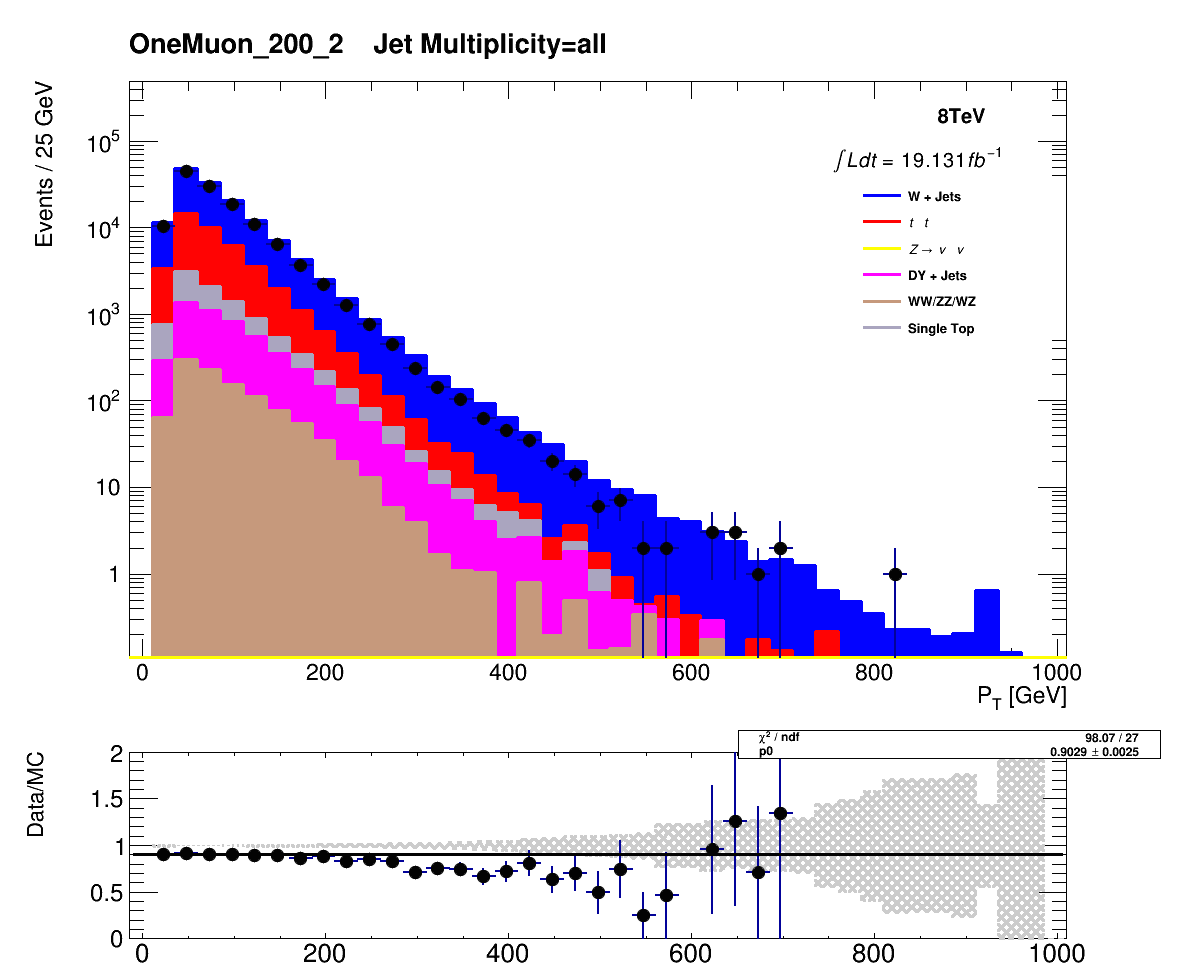
\includegraphics[width=\textwidth]{Figs/datamc/mu/Stacked_MuPt_all_OneMuon_200_upwards}
      \caption{$\mu$ \Pt}
    \end{subfigure}
    \begin{subfigure}[b]{0.48\textwidth}
      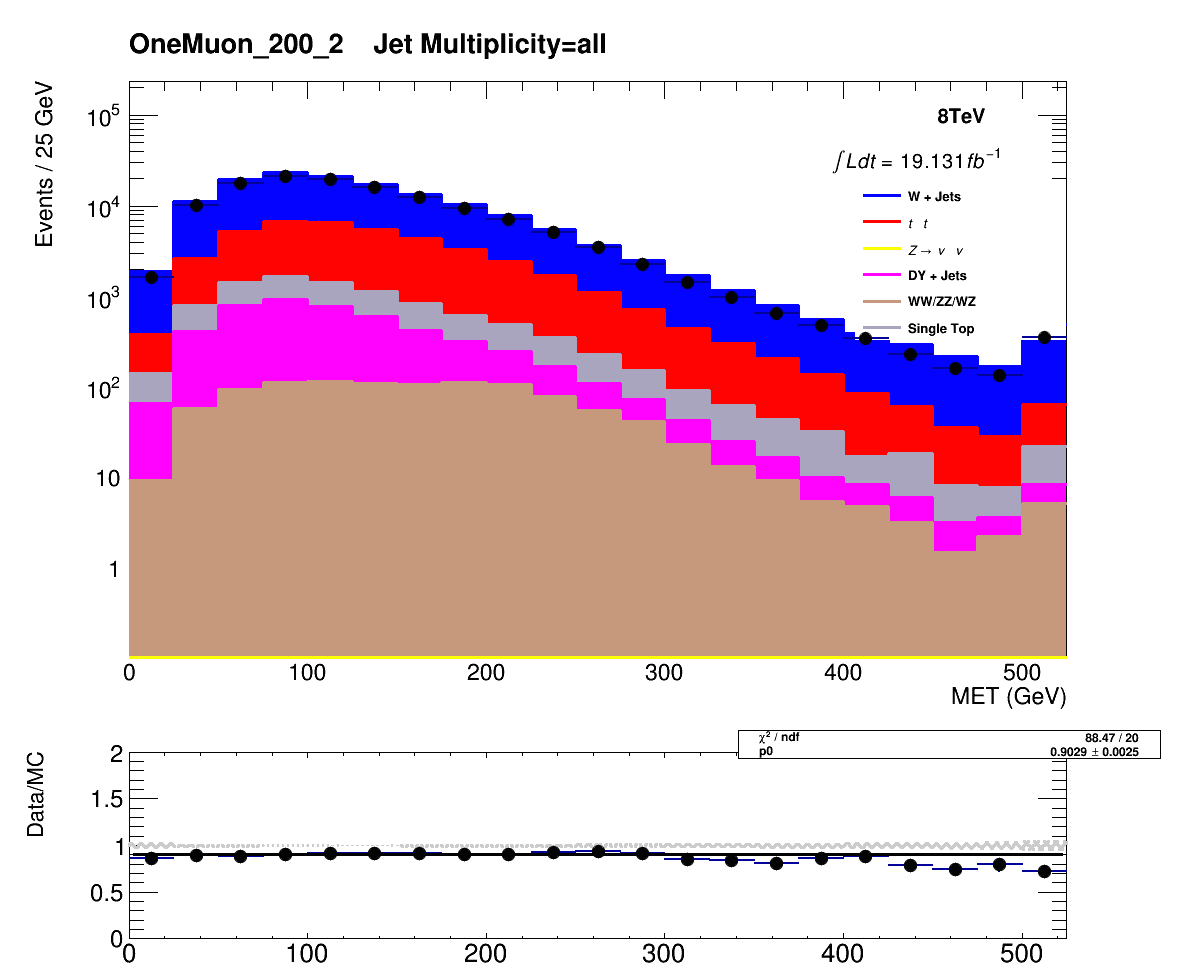
\includegraphics[width=\textwidth]{Figs/datamc/mu/Stacked_MET_Corrected_all_OneMuon_200_upwards}
      \caption{\met (corrected for $\mu$)}
    \end{subfigure} \\
    \caption{\label{fig:datamc_mu_inc}
    Comparison of data with MC for the \mj control selection. Plots 
    are for $\HT>200$ \gev, $\nj\geq2, \nb\geq0$.
    }
\end{figure}


\subsection{\mmj}
The \mmj sample is constructed to predict background contributions from \zinv 
decays, mimicking this decay via the kinematically similar $Z\to\mu\mu + jets$
process where both muons are subsequently ignored.
The sample is used to provide low \HT coverage for the \zinv background 
prediction, where the \gj sample (section~\ref{sec:gjets_control_sample})
is unable to do so.

\subsubsection{Triggers}
The trigger used is the same as for the \mj sample, as described in
section~\ref{sec:mujets_control_trigger}. Trigger efficiencies are significantly
improved for the dimuon selection given that either of the muons 
can cause a positive trigger decision, as shown in table~\ref{tab:dimuon-trig-effs}. 
Relative errors are considered the same as for the \mj trigger efficiencies.

\begin{table}[!ht]
  \caption{Muon trigger efficiencies (\%) for the \mmj selection listed by
  \HT bin and \nj category.}
  \label{tab:dimuon-trig-effs}
  \centering
  \small
  \begin{tabular}{ cccc }
    \hline
    \hline
    \HT (GeV) & 2-3 & $\geq$4 \\ [0.5ex]
                                       
    \hline
    150--200  & 98.4 & 98.4  \\
    200--275  & 98.5 & 98.4  \\
    275--325  & 98.5 & 98.4  \\
    325--375  & 98.6 & 98.6  \\
    375--475  & 98.6 & 98.5  \\
    475--575  & 98.6 & 98.6  \\
    575--675  & 98.6 & 98.6  \\
    675--775  & 98.7 & 98.6  \\
    775--875  & 98.6 & 98.6  \\
    875--975  & 98.7 & 98.6  \\
    975--1075 & 98.7 & 98.8  \\
    $>$1075   & 98.7 & 98.7  \\
    \hline
    \hline
  \end{tabular}
\end{table}

\subsubsection{Selection Criteria}
The selection for the \mmj sample is very similar to that of the \mj sample, 
described in section~\ref{sec:mujets_control_selection}, with differences chosen
to enrich the sample in Z bosons decaying to pairs of muons in the kinematic 
phase space of the signal region. Two tight isolated muons are selected, each 
with $\Pt > 30$ \gev and $|\eta| < 2.1$. Their invariant mass is chosen to be
tight around $m_Z$, $m_Z - 25 < M_{\mu_1\mu_2} < m_Z + 25$ \gev. Furthermore, a 
veto is made on events satisfying $\Delta R(\mu_i, jet_j) < 0.5$, for every muon 
$i$ and every jet $j$. Similarly as in the \mj sample selection, no \alphat
requirement is made.

Example distributions of $M_T(\mu\mu)$ and $\mu_2$ \Pt for this selection are
shown in figure~\ref{fig:datamc_mumu_inc}.

\begin{figure}[!ht]
  \centering
    \begin{subfigure}[b]{0.48\textwidth}
      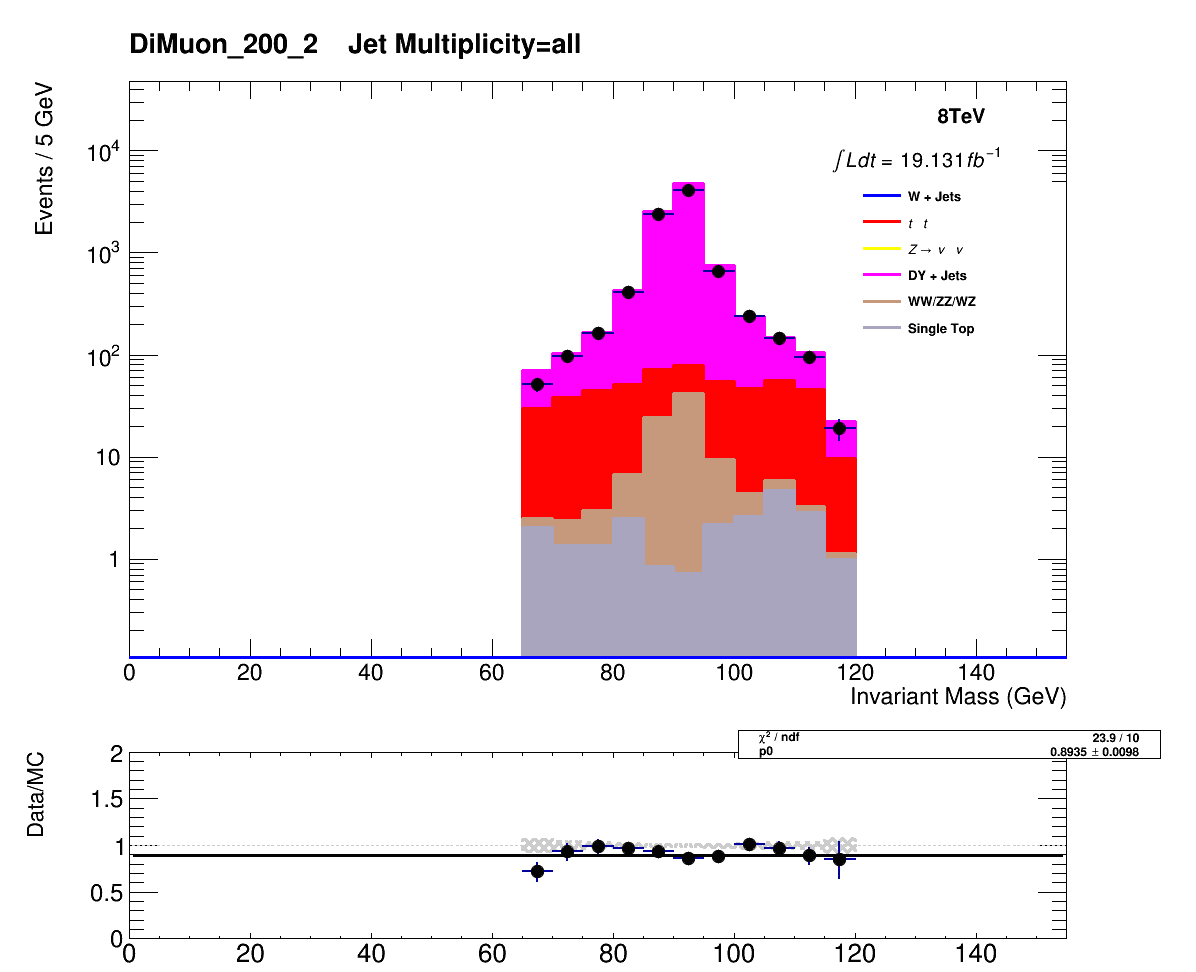
\includegraphics[width=\textwidth]{Figs/datamc/mumu/Stacked_DiMuon_Mass_all_DiMuon_200_upwards}
      \caption{$M_T(\mu, \mu)$}
    \end{subfigure}
    \begin{subfigure}[b]{0.48\textwidth}
      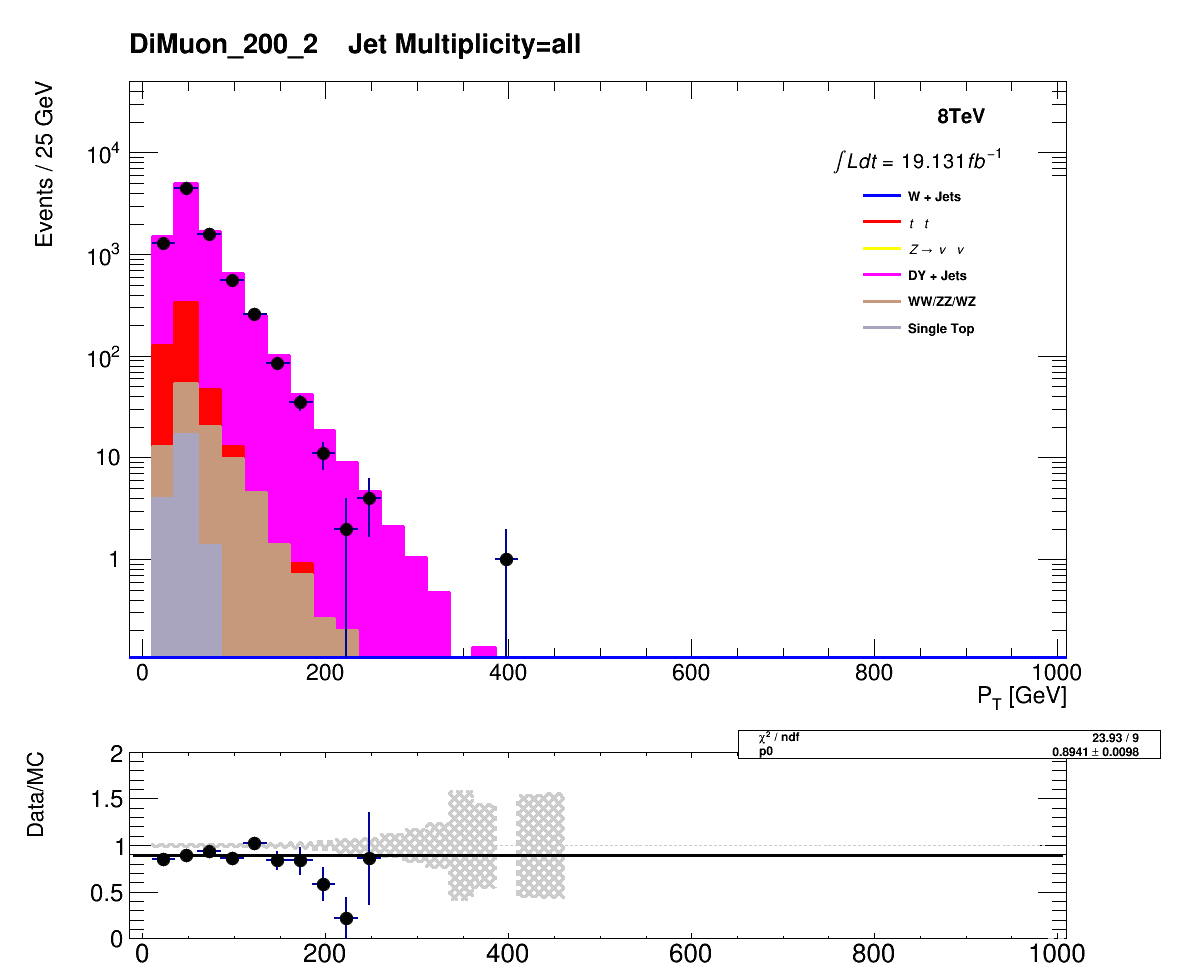
\includegraphics[width=\textwidth]{Figs/datamc/mumu/Stacked_SecondMuPt_all_DiMuon_200_upwards}
      \caption{Second $\mu$ \Pt}
    \end{subfigure} \\
    \caption{\label{fig:datamc_mumu_inc}
    Comparison of data with MC for the \mmj control selection. Plots 
    are for $\HT>200$ \gev, $\nj\geq2, \nb\geq0$.}
\end{figure}

\subsection{\gj}
\label{sec:gjets_control_sample}
The \gj sample is used to predict the \zinv background contribution, given it's 
similar kinematics when the $\gamma$ is ignored from the event, and larger 
production cross section relative to \mmj. Due to trigger thresholds, the \gj
sample cannot make predictions for $\HT<375$ \gev, and so is complimentary to
the \mmj sample prediction.

\subsubsection{Triggers}
Events are collected using the \verb!HLT_Photon150! trigger. The trigger's 
efficiency is measured using the \verb!HLT_Photon90! trigger as a reference and
is found to be 100$\%$ efficient for $E_T^{photon}>165\gev$ and $\HT>375$ \gev, 
as shown by the turn on curves in figure~\ref{fig:photon_control_trigeff}.

\begin{figure}[ht!]
  \centering
  \begin{subfigure}[b]{0.35\textwidth}
    \includegraphics[width=\textwidth, page=3,trim=40 40 160 120,clip=true]{figures/trigger/g_barrel_375_caloJet_le3j.pdf}
    \caption{\njlow}
    \label{fig:photon_control_trigeff_le3j}
  \end{subfigure}
  \begin{subfigure}[b]{0.35\textwidth}
    \includegraphics[width=\textwidth, page=3,trim=40 40 160 120,clip=true]{figures/trigger/g_barrel_375_caloJet_ge4j.pdf}
    \caption{\njhigh}
    \label{fig:photon_control_trigeff_ge4j}
  \end{subfigure}
  \caption{Efficiency turn-on curves for the photon trigger, based on the \gj 
  selection, for \HT > 375 \gev, with \njlow (Left) and \njhigh(Right).}
  \label{fig:photon_control_trigeff}
\end{figure}

\subsubsection{Selection Criteria}
Exactly one photon satisfying tight isolation criteria is required, with 
$\Pt > 165$ \gev and $|\eta|<1.45$. In addition, events are vetoed if
$\Delta R(\gamma, jet_i)<1.0$ is satisfied, for all of the events $i$ jets.

An example distribution of the $\gamma$ \Pt for this selection is shown
in figure~\ref{fig:datamc_pho_inc}.

\begin{figure}[!ht]
  \centering
    \begin{subfigure}[b]{0.48\textwidth}
      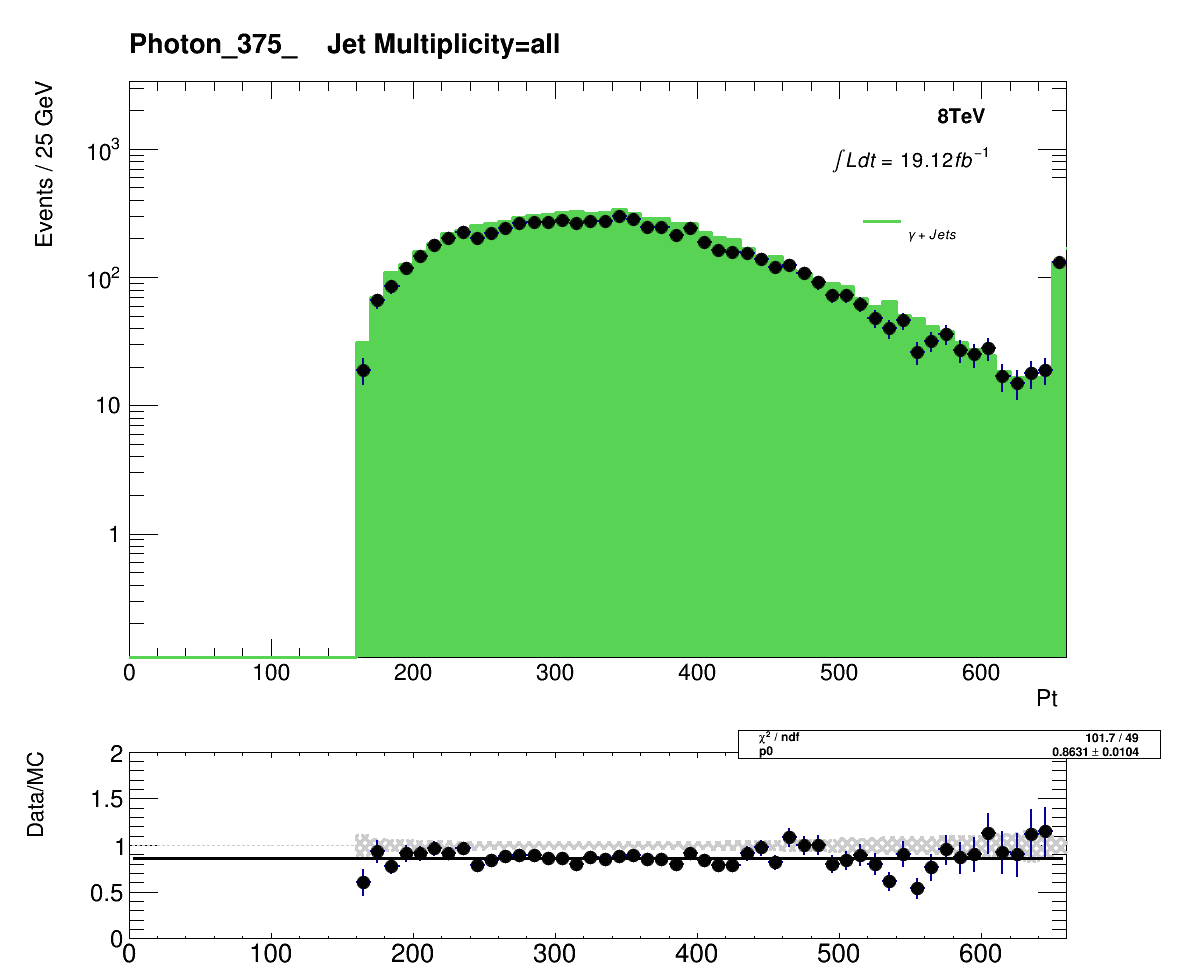
\includegraphics[width=\textwidth]{Figs/datamc/pho/Stacked_PhotonPt_all_Photon_375_upwards}
      \caption{$\gamma$ $\Pt$}
    \end{subfigure}
    \caption{\label{fig:datamc_pho_inc}
    Comparison of data with MC for the \gj control selection. Plot 
    is for $\HT>200$ \gev, $\nj\geq2, \nb\geq0$.}
\end{figure}

%********************************** % Third Section  *************************************
% \section{Estimating multijet backgrounds}  %Section - 1.3
% \label{sec:background_qcd}

% A data-driven technique has been developed to measure any remaining QCD events
% in the signal region. This is used to determine a \HT dependent \alphat
% requirement such that QCD is at the sub-percent level with respect to the total
% EWK background.

% \subsection{Multijet control sample}
% In order to predict the contamination of QCD MJ events in the signal region a 
% control region of hadronic events is constructed.

% \subsubsection{Triggers}
% Events are collected using a suite of triggers requiring various thresholds of 
% \HT. By using single-object \HT triggers it is possible to study events
% across a spectrum of \alphat values. The high rates expected through these
% triggers were maintained throughout
% the 2012 run with a variety of prescales. Each trigger seeds a single \HT bin in
% the analysis, with a 25 \gev offset between the online trigger requirement and 
% the offline threshold. Efficiencies are measured with the same technique as the
% signal triggers, using the \verb!HLT_IsoMu24_eta2p1! trigger as a reference. 
% The efficiencies of these triggers are summarised in table~\ref{tab:ht-triggers}.

% \begin{table}[!ht]
%   \caption{List of \texttt{HTxxx} triggers and their efficiencies
%     (\%), as measured in data for each \HT bin and \nj category. Also listed are
%     the typical prescales applied and the L1 seed triggers.}
%   \label{tab:ht-triggers}
%   \centering
%   \scriptsize
%   \begin{tabular}{ ccccll }
%     \hline
%     \hline
%     Offline \HT & L1 seed (\verb!L1_?!) & Trigger (\verb!HLT_?!) &    Typical & \multicolumn{2}{c}{Efficiency (\%)}\\ [0.5ex]
%    region (\gev) & (highest thresholds) &  & prescale & \multicolumn{1}{c}{$2 \leq \nj \leq 3$} & \multicolumn{1}{c}{$\nj \geq 4$} \\ [0.5ex]

%     \hline
%     $200 < \HT < 275$  & \verb!DoubleJetC64!           & \verb!HT250! & 4800     & $\phantom{1}66.4 \pm 14.1$                & $154.3 \pm 154.3$                     \\
%     $275 < \HT < 325$  & \verb!DoubleJetC64 OR HTT175! & \verb!HT250! & 2400     & $\phantom{1}97.3 \pm 23.0$                & $\phantom{1}91.7 \pm \phantom{1}53.1$ \\
%     $325 < \HT < 375$  & \verb!DoubleJetC64 OR HTT175! & \verb!HT300! & 1200     & $\phantom{1}79.5 \pm 20.6$                & $198.1 \pm \phantom{1}81.2$           \\
%     $375 < \HT < 475$  & \verb!DoubleJetC64 OR HTT175! & \verb!HT350! & 600      & $108.7 \pm 18.7$                          & $\phantom{1}54.5 \pm \phantom{1}31.6$ \\
%     $475 < \HT < 575$  & \verb!DoubleJetC64 OR HTT175! & \verb!HT450! & 150      & $110.6 \pm 15.9$                          & $106.4 \pm \phantom{1}26.8$           \\
%     $575 < \HT < 675$  & \verb!DoubleJetC64 OR HTT175! & \verb!HT550! & 70       & $\phantom{1}96.1 \pm 14.7$                & $104.4 \pm \phantom{1}23.1$           \\
%     $675 < \HT < 775$  & \verb!DoubleJetC64 OR HTT175! & \verb!HT650! & 25       & $\phantom{1}94.3 \pm 15.4$                & $101.2 \pm \phantom{1}21.5$           \\
%     $775 < \HT < 875$  & \verb!DoubleJetC64 OR HTT175! & \verb!HT750! & 1        & $\phantom{1}96.9 \pm \phantom{1}6.1$      & $\phantom{1}94.4 \pm \phantom{11}8.3$ \\
%     $875 < \HT < 975$  & \verb!DoubleJetC64 OR HTT175! & \verb!HT750! & 1        & $100.0 \pm \phantom{1}8.4$                & $100.0 \pm \phantom{1}12.6$           \\
%     $975 < \HT < 1075$ & \verb!DoubleJetC64 OR HTT175! & \verb!HT750! & 1        & $100.0 \pm 11.2$                          & $100.0 \pm \phantom{1}15.3$           \\
%     $\HT > 1075$       & \verb!DoubleJetC64 OR HTT175! & \verb!HT750! & 1        & $100.0 \pm 15.0$                          & $100.0 \pm \phantom{1}22.9$           \\
%     \hline
%     \hline
%   \end{tabular}
% \end{table}

% \subsubsection{Selection Criteria}
% The selection of this sample matches that of the hadronic signal region, with 
% the exception that both the \alphat and \mhtmet requirements are removed 
% ensuring a very high yield of QCD MJ events.


% \subsection{Prediction Technique}

% Events from the hadronic control sample are used to populate a plane of \mhtmet 
% and \alphat. A prediction of the EWK contribution to this sample is determined 
% from the \mj control sample with the \mhtmet requirement removed, using the TF 
% factor method described in section~\ref{sec:background_overview}. The prediction
% is subtracted from the hadronic control sample yields as a function of \mhtmet
% and \alphat, leaving a pure sample of QCD MJ events (SHOW PLOTS?).

% By considering events both above and below the nominal \mhtmet threshold of
% 1.25, the ratio \rmhtmet is constructed, defined as:
% % 
% \begin{equation}
% \label{eq:rmhtmet}
% \rmhtmet = \frac{N(\mhtmet<1.25)}{N(\mhtmet>1.25)}
% \end{equation}

% A fit is made to this variable as a function of \alphat, using an exponential 
% functional form:
% % 
% \begin{equation}
% \label{eq:fit_exp}
% \rmhtmet(\alphat) = e^{{-(a+b.\alphat)}^n}
% \end{equation}
% % 
% both for $n=0$ and also when $n$ is allowed to float as a free 
% parameter within the range $0-2$ in order to span the scenarios from flat to a
% Gaussian form. Example distributions and fits are shown in FIGURE.

% QCD yield predictions are made and compared with the relevant EWK background 
% contributions in table~\ref{tab:qcd-pred-data}. \alphat thresholds are chosen 
% for each \HT bin such that the ratio of QCD to EWK is at the sub-percent level. 
% The chosen \alphat threshold values are summarised in
% table~\ref{tab:alphat_thresholds_qcd}.

% \begin{table}[h!]
% \centering
% \scriptsize
%   \caption{QCD multijet background contribution prediction summarised for the 
%   main analysis categories of \nb, \nj and \HT as a function of \alphat. The 
%   predicted EWK background contribution is included for comparison, and a 
%   the ratio of QCD/EWK is also shown.}
% \label{tab:qcd-pred-data}
% \begin{tabular}{ccccrrr}
% \hline
% \hline
% \nj & \nb & \HT (GeV) & Bkgd & \multicolumn{3}{c}{\alphat threshold} \\
% \cline{5-7}
%  & & & & \multicolumn{1}{c}{0.550}   & \multicolumn{1}{c}{0.600}   & \multicolumn{1}{c}{0.650} \\
% \hline
% 2--3 & 0 & 200--275 & QCD  & $\left(3.8 \pm 1.3 \pm 1.2 \right) \times 10^{3}$ & $\left(4.1 \pm 2.4 \pm 3.0 \right) \times 10^{1}$ & $\left(0.9 \pm 0.8 \pm 1.5 \right) \times 10^{0}$\\
% 2--3 & 0 & 200--275 & EWK  & $\left(2.1 \pm 0.1\right) \times 10^{4}$ & $\left(1.5 \pm 0.0\right) \times 10^{4}$ & $\left(1.2 \pm 0.0\right) \times 10^{4}$\\
% 2--3 & 0 & 200--275 & Ratio  & $0.2 \pm 0.1$ & $0.003 \pm 0.003$ & $0.0001 \pm 0.0001$\\ [1.0ex]
% 2--3 & 0 & 275--325 & QCD  & $\left(1.0 \pm 0.3 \pm 1.5 \right) \times 10^{4}$ & $\left(0.2 \pm 0.1 \pm 0.7 \right) \times 10^{0}$ & $\left(0.8 \pm 0.3 \pm 4.8 \right) \times 10^{-3}$\\
% 2--3 & 0 & 275--325 & EWK  & $\left(7.9 \pm 0.2\right) \times 10^{3}$ & $\left(5.3 \pm 0.2\right) \times 10^{3}$ & $\left(4.0 \pm 0.2\right) \times 10^{3}$\\
% 2--3 & 0 & 275--325 & Ratio  & $1 \pm 2$ & $0.0000 \pm 0.0001$ & $\left(0 \pm 1\right) \times 10^{-6}$\\ [1.0ex]
% 2--3 & 0 & 325--375 & QCD  & $\left(2.8 \pm 0.4 \pm 2.1 \right) \times 10^{1}$ & $\left(0.9 \pm 0.2 \pm 1.3 \right) \times 10^{-1}$ & $\left(0.6 \pm 0.4 \pm 1.2 \right) \times 10^{-3}$\\
% 2--3 & 0 & 325--375 & EWK  & $\left(3.4 \pm 0.1\right) \times 10^{3}$ & $\left(2.2 \pm 0.1\right) \times 10^{3}$ & $\left(1.7 \pm 0.1\right) \times 10^{3}$\\
% 2--3 & 0 & 325--375 & Ratio  & $0.008 \pm 0.006$ & $\left(4 \pm 6\right) \times 10^{-5}$ & $\left(4 \pm 8\right) \times 10^{-7}$\\ [1.0ex]
% $\geq 4$ & 0 & 200--275 & QCD  & $\left(2.8 \pm 1.5 \pm 1.3 \right) \times 10^{3}$ & $\left(1.1 \pm 0.7 \pm 0.2 \right) \times 10^{1}$ & $\left(0.2 \pm 0.2 \pm 0.0 \right) \times 10^{0}$\\
% $\geq 4$ & 0 & 200--275 & EWK  & $\left(4.3 \pm 0.3\right) \times 10^{2}$ & $\left(2.0 \pm 0.1\right) \times 10^{2}$ & $\left(1.0 \pm 0.1\right) \times 10^{2}$\\
% $\geq 4$ & 0 & 200--275 & Ratio  & $7 \pm 5$ & $0.06 \pm 0.04$ & $0.002 \pm 0.002$\\ [1.0ex]
% $\geq 4$ & 0 & 275--325 & QCD  & $\left(1.5 \pm 1.2 \pm 1.0 \right) \times 10^{4}$ & $\left(1.5 \pm 1.7 \pm 0.3 \right) \times 10^{0}$ & $\left(0.1 \pm 0.2 \pm 0.0 \right) \times 10^{-1}$\\
% $\geq 4$ & 0 & 275--325 & EWK  & $\left(1.2 \pm 0.0\right) \times 10^{3}$ & $\left(5.3 \pm 0.2\right) \times 10^{2}$ & $\left(2.9 \pm 0.1\right) \times 10^{2}$\\
% $\geq 4$ & 0 & 275--325 & Ratio  & $\left(1 \pm 1\right) \times 10^{1}$ & $0.003 \pm 0.003$ & $\left(4 \pm 7\right) \times 10^{-5}$\\ [1.0ex]
% $\geq 4$ & 0 & 325--375 & QCD  & $\left(0.7 \pm 0.1 \pm 0.8 \right) \times 10^{0}$ & $\left(2.5 \pm 0.6 \pm 6.5 \right) \times 10^{-5}$ & $\left(0.7 \pm 0.3 \pm 2.8 \right) \times 10^{-8}$\\
% $\geq 4$ & 0 & 325--375 & EWK  & $\left(4.8 \pm 0.3\right) \times 10^{2}$ & $\left(2.0 \pm 0.1\right) \times 10^{2}$ & $\left(1.1 \pm 0.1\right) \times 10^{2}$\\
% $\geq 4$ & 0 & 325--375 & Ratio  & $0.002 \pm 0.002$ & $\left(1 \pm 3\right) \times 10^{-7}$ & $\left(1 \pm 3\right) \times 10^{-10}$\\ [1.0ex]
% %2--3 & $\geq 1$ & 200--275 & QCD  & $\left(2.2 \pm 1.1 \pm 4.5 \right) \times 10^{2}$ & $\left(0.5 \pm 0.2 \pm 3.2 \right) \times 10^{0}$ & $\left(0.3 \pm 0.1 \pm 4.5 \right) \times 10^{-2}$\\
% %2--3 & $\geq 1$ & 200--275 & EWK  & $\left(3.7 \pm 0.1\right) \times 10^{3}$ & $\left(2.5 \pm 0.1\right) \times 10^{3}$ & $\left(1.9 \pm 0.1\right) \times 10^{3}$\\
% %2--3 & $\geq 1$ & 200--275 & Ratio  & $0.1 \pm 0.1$ & $0.000 \pm 0.001$ & $\left(0 \pm 2\right) \times 10^{-5}$\\ [1.0ex]
% \hline
% \hline
% \end{tabular}
% \end{table}

% \emph{RELATED SYSTEMATICS?}

% \begin{table}[!ht]
%   \caption{\alphat thresholds for each analysis \HT bin as determined from the 
%   QCD MJ prediction method, such that QCD is at the sub-percent level.}
%   \label{tab:alphat_thresholds_qcd}
%   \centering
%   \small
%   \begin{tabular}{ cc }
%     \hline
%     \hline
%     \HT (GeV) & \alphat threshold \\ [0.5ex]
                                       
%     \hline
%     200--275  & 0.65 \\
%     275--325  & 0.60 \\
%     >325  & 0.55 \\
%     \hline
%     \hline
%   \end{tabular}
% \end{table}


%********************************** % Fifth Section  *************************************
\section{Background control and systematic uncertainties on SM background predictions}  %Section - 1.5
\label{sec:background_systematics}

In order to probe the levels at which the transfer factors are sensitive to 
relevant uncertainties, a statistically powerful ensemble of Closure Tests
(CT's) have been designed. The CT method works by constructing a TF to
extrapolate from one sub-region of a particular control sample into another 
control sample sub-region. In doing so, tests can be designed to specifically 
probe any potential sources of bias in the transfer factors.

\subsection{Closure tests}
\label{sec:closure_tests}

Closure tests are performed as a function of \HT, in the two \nj categories,
\njlow and \njhigh. The level of closure represents the statistical 
consistency between predicted and observed yields for each test, in the absence 
of any assumed systematic uncertainty. The test statistic is defined as $(N_{obs}
- N_{pred}) / N_{pred}$, with any bias being observed as a statistically 
significant deviation from zero, or a trend in \HT.

\begin{figure}[ht!]
  \centering
  \begin{subfigure}[b]{0.7\textwidth}
    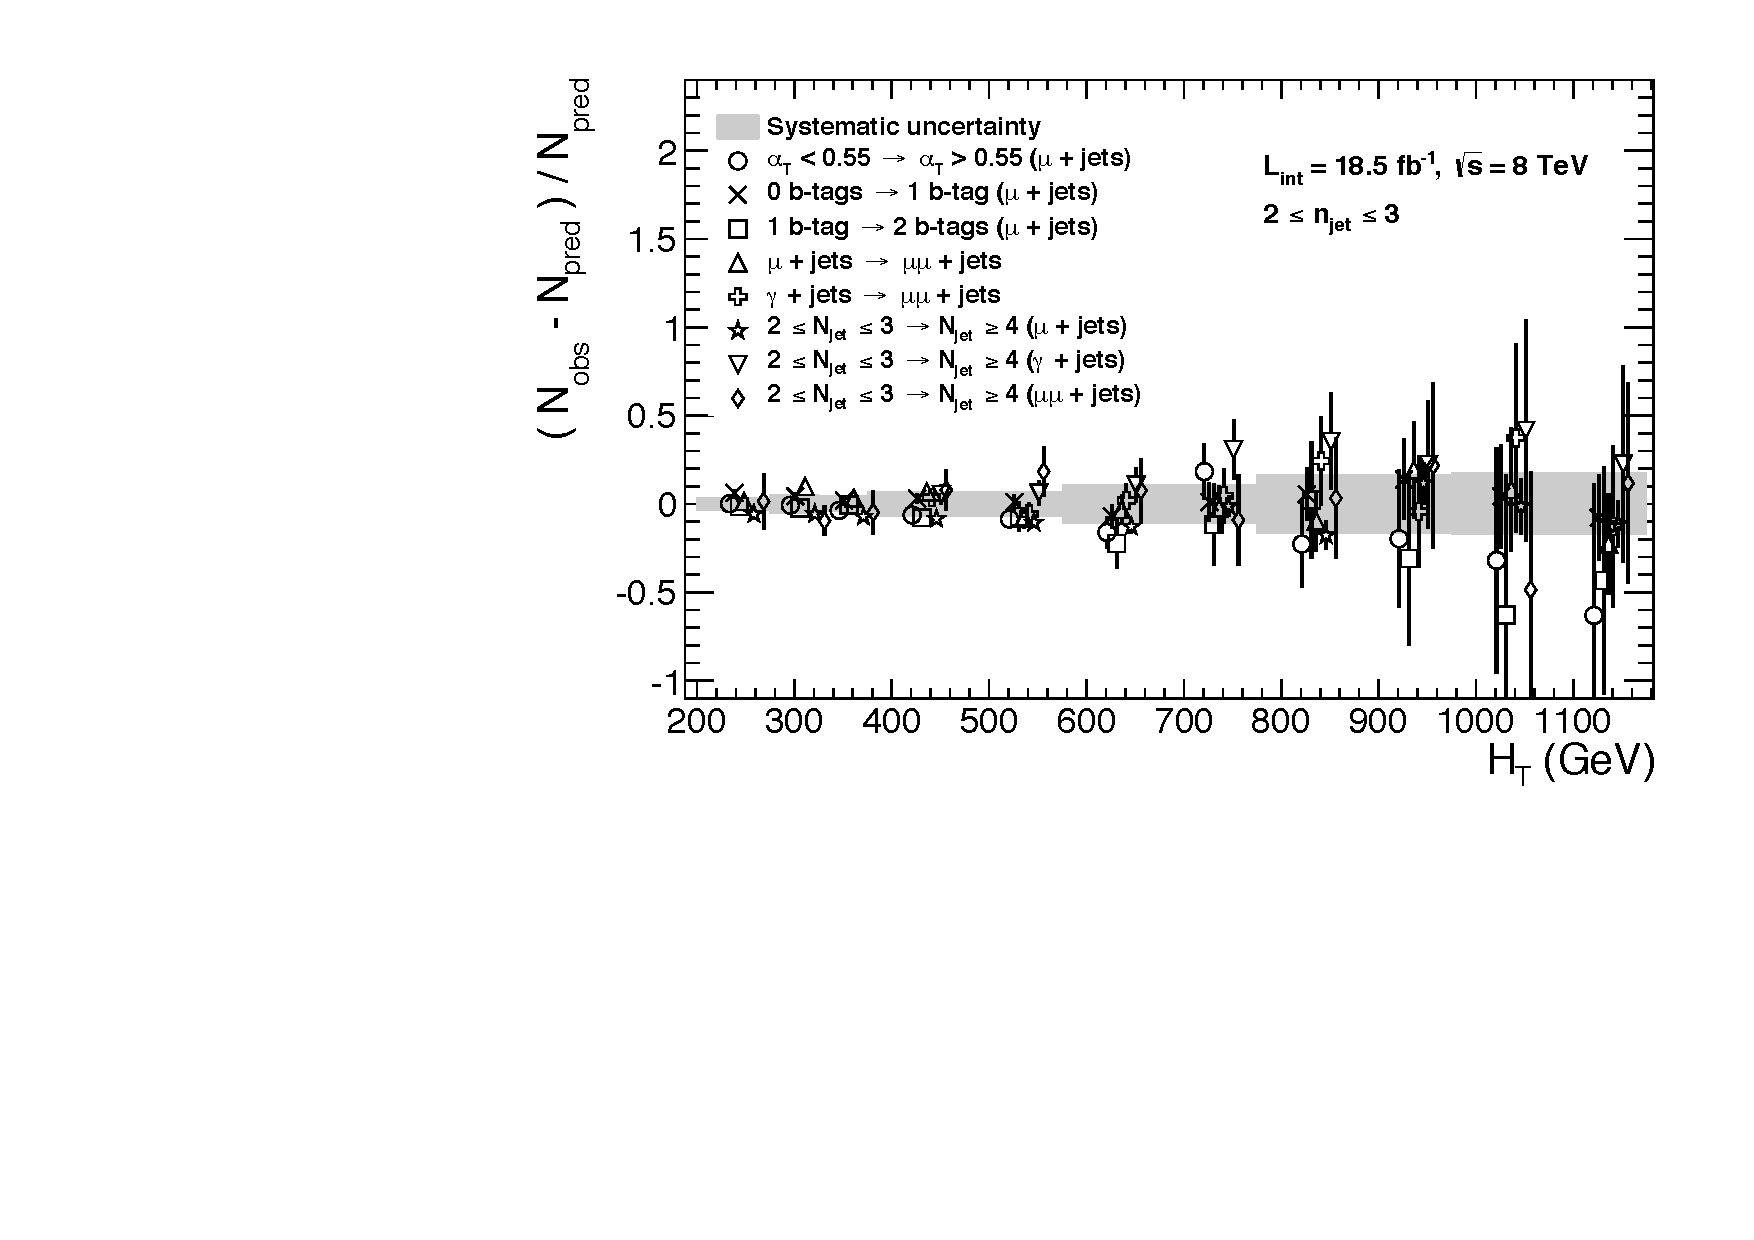
\includegraphics[width=\textwidth]{Figs/syst/v0/le3j/summary_plot}
    \caption{$2 \leq \nj \leq 3$}
    \label{fig:closure_summary_le3j}
  \end{subfigure}             
  \begin{subfigure}[b]{0.7\textwidth}
    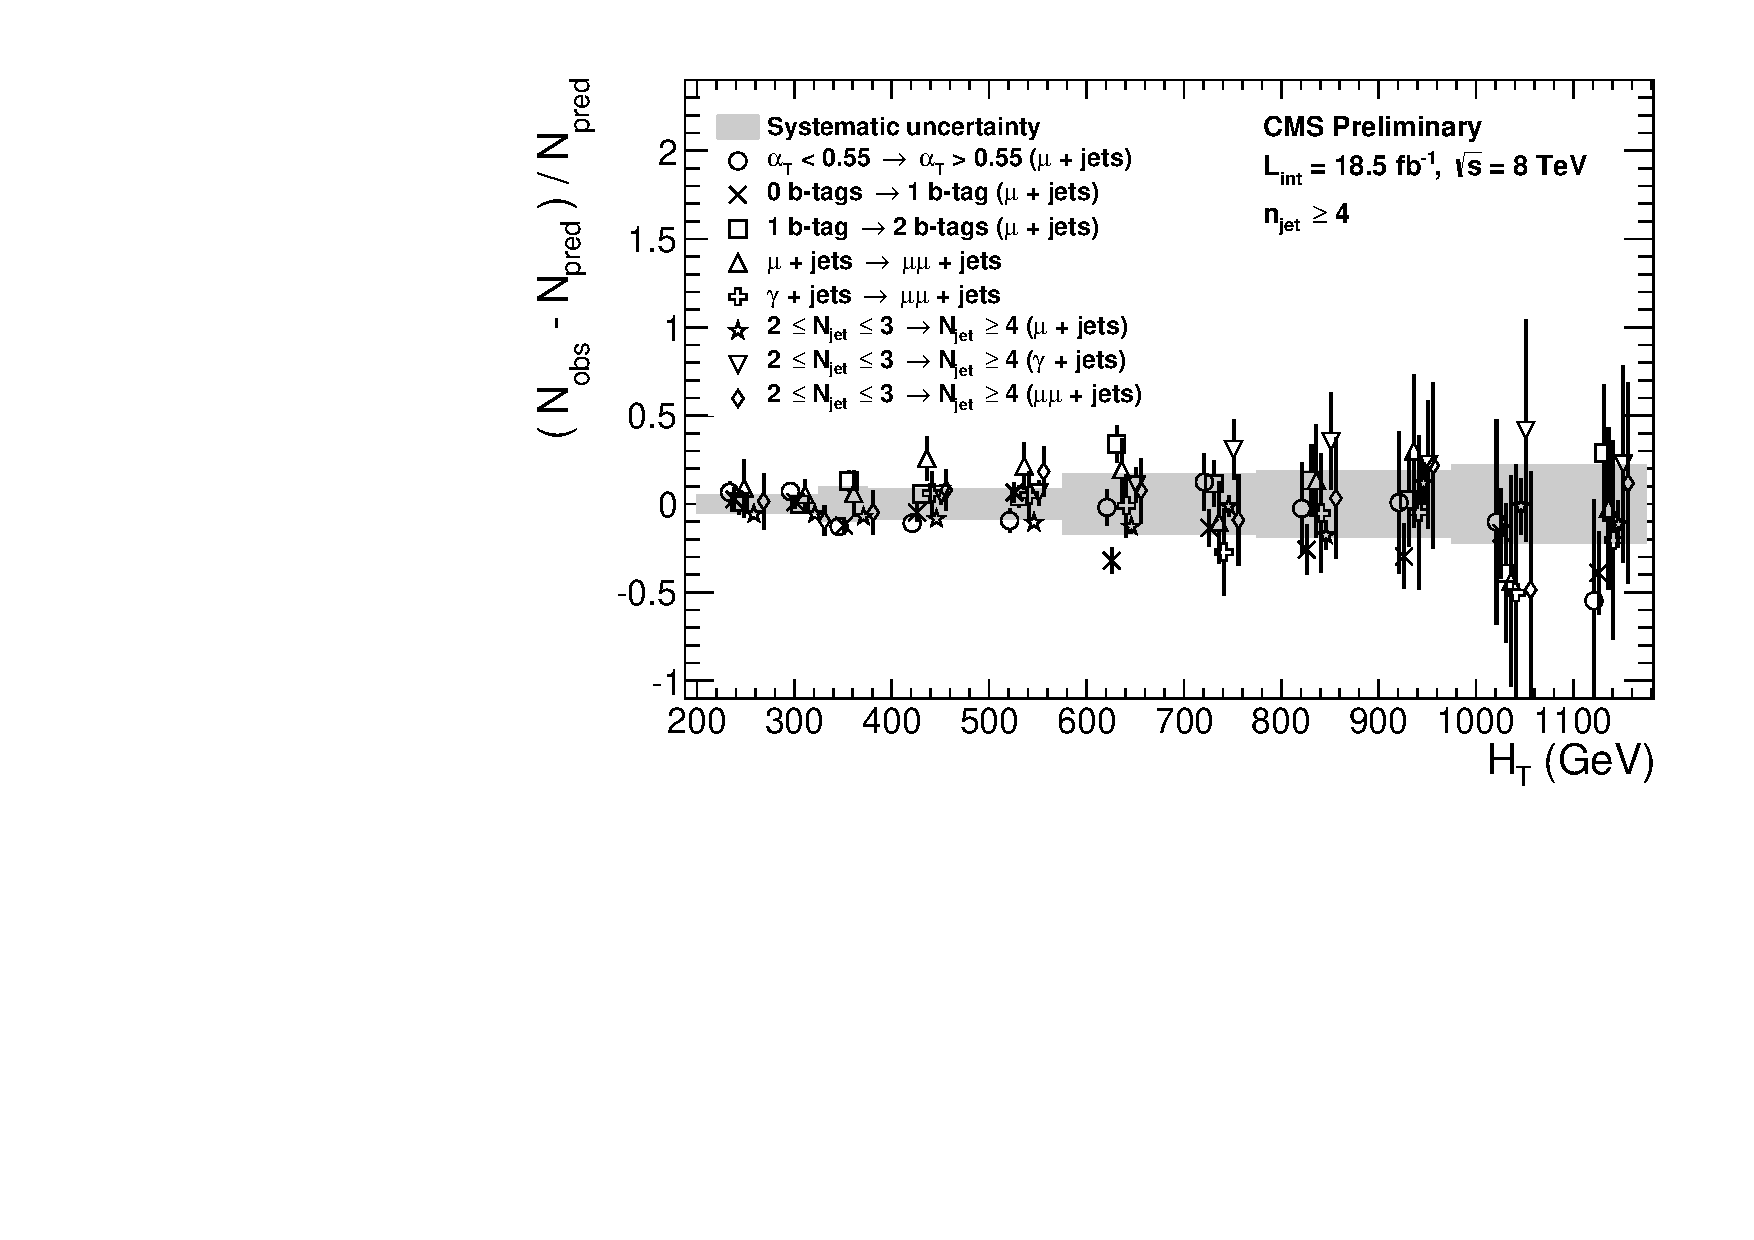
\includegraphics[width=\textwidth]{Figs/syst/v0/ge4j/summary_plot}
    \caption{$\nj \geq 4$}
    \label{fig:closure_summary_ge4j}
  \end{subfigure}             
  % \caption{Sets of closure tests (open symbols) overlaid on top of
  %     the systematic uncertainty used for each of the five \HT
  %     regions (shaded bands) and for the two different jet
  %     multiplicity bins: (a) $2 \leq \nj \leq 3$ and (b) $\nj \geq
  %     4$. RE}
  \caption{The results of the eight core closure tests (open symbols), shown 
  over the systematic uncertainty bands for each of the five \HT regions
  (shaded grey), for the two jet multiplicity regions (a) \njlow and (b) \njhigh 
  seperately.}
  \label{fig:closure_summary}
\end{figure}

Figure~\ref{fig:closure_summary} shows a summary of the eight closure tests 
considered as `core' tests for the analysis, split into both
\njlow (figure~\ref{fig:closure_summary_le3j}) 
and \njhigh (figure~\ref{fig:closure_summary_ge4j}). It should be noted that 
numerous other tests are also considered, but that these eight represent those 
deemed most important to the background prediction uncertainty.

The first test, represented by open circles, tests the modelling of the \alphat 
variable in the \mj control sample. In the analysis a prediction is made 
between the \mj sample, which has no \alphat requirement, and the 
signal region, with it's tight \alphat requirement. This particular test probes
the validity of predicting between the `bulk' of the \alphat distribution in the
control sample
and the `tail' of the distribution in the signal region. A similar test, not
shown here, is performed for the \mmj control sample.

The next two tests, represented by crosses and open squares, probe the
different b-tag multiplicities in the \mj control sample. The b-tag 
requirements greatly change the relative admixture of, for example, \wj (\nb=0)
and \ttj (\nb=1) events.
It is important to note that this test is 
considered conservative, given that the admixture of \wj to \ttj events 
varies minimally between control and signal regions, where this extrapolation is 
made in the analysis. Given the focus on b-tagging, these tests also investigate
the modelling of b-quark jets in the simulated data.

A similar test is made for the relative admixture of \zj to \wj and \ttj, by 
predicting between the \mj and \mmj control regions, represented by open 
triangles. Again, this test is considered 
conservative, but also probes the muon reconstruction and trigger efficiencies 
between the different muon multiplicities. These are however already well 
studied by the muon \emph{POG} using data-driven techniques.

As described in section~\ref{sec:background_overview}, the \zinv prediction 
is made from both the \gj and \mmj samples, and so a test is constructed to 
predict between these two orthogonal control regions, as shown by the open 
crosses.

The final three tests, indicated by open stars, triangles and diamonds, make 
predictions between the two different jet multiplicity categories in each 
control sample, thereby 
testing jet reconstruction and modelling. This test is also considered very 
conservative as the analysis only predicts between identical \nj categories in 
the control and signal regions.

Summary plots of these eight tests are shown in
figure~\ref{fig:closure_summary}, indicating that there are no statistically
significant biases
or \HT dependencies. Figures~\ref{fig:closure_fit_le3j_pol0} and \ref{fig:closure_fit_ge4j_pol0} show
zeroeth order polynomial fits (blue lines) made to each individual test to assess the 
level of any potential bias present. In addition, first order polynomial fits 
(red lines) are
also made to assess any potential \HT dependence present in the tests, as shown
in figures~\ref{fig:closure_fit_le3j_pol1} and \ref{fig:closure_fit_ge4j_pol1}.
The best-fit values, $\chi^2$ and $p$-values 
obtained from both fits are summarised for each \nj category in
tables~\ref{tab:syst-fits-le3j}, \ref{tab:syst-fits-ge4j} and
\ref{tab:syst-fits-njet}.

As expected, the fits show no significant biases or trends, and therefore 
indicate good closure. The only exception is the 0 b-jets \ra 1 b-jet (\mj) test
for the \njhigh category
which has a sub-optimal goodness of fit value. This is 
attributed to upwards and downwards fluctuations in the 475-575 \gev and 575-675
\gev bins respectively. Also shown in table~\ref{tab:syst-fits-ge4j}, when the 
same fit is made after summing these two bins significantly improved fit
parameters are observed. This leads to the conclusion that these two
bins contain a statistical fluctuation as opposed to a systematic bias.

\begin{figure}[ht!]
  \centering
  \begin{subfigure}[b]{0.46\textwidth}
    \includegraphics[width=\textwidth]{figures/syst/v0/le3j/summary_plot_pol0}
    \caption{$2 \leq \nj \leq 3$ (constant function fits)}
    \label{fig:closure_fit_le3j_pol0}
  \end{subfigure}
  \begin{subfigure}[b]{0.46\textwidth}
    \includegraphics[width=\textwidth]{figures/syst/v0/le3j/summary_plot_pol1}
    \caption{$2 \leq \nj \leq 3$ (linear function fits)}
    \label{fig:closure_fit_le3j_pol1}
  \end{subfigure}
  \begin{subfigure}[b]{0.46\textwidth}
    \includegraphics[width=\textwidth]{figures/syst/v0/ge4j/summary_plot_pol0}
    \caption{$\nj \geq 4$ (constant function fits)}
    \label{fig:closure_fit_ge4j_pol0}
  \end{subfigure}
  \begin{subfigure}[b]{0.46\textwidth}
    \includegraphics[width=\textwidth]{figures/syst/v0/ge4j/summary_plot_pol1}
    \caption{$\nj \geq 4$ (linear function fits)}
    \label{fig:closure_fit_ge4j_pol1}
  \end{subfigure}
  \caption{The results of the eight core closure tests (open symbols), shown 
  over the systematic uncertainty bands for each of the five \HT regions
  (shaded grey), for the two jet multiplicity regions (a) \njlow and (b) \njhigh 
  seperately. Included are zeroeth order (left column, blue) and first order (right 
  column, red) fits to each individual closure test.}
  \label{fig:closure_fits}
\end{figure}

\begin{table}[!ht]
  \caption{Results of zeroeth (i.e. constant) and first order (i.e. linear) fits
  for five sets of closure tests, performed in the \njlow category.}
  \label{tab:syst-fits-le3j}
  \centering
  \tiny
  \begin{tabular}{ llrccccrc }
    \hline
    \hline
                                              &          & \multicolumn{4}{c}{Constant fit} &          & \multicolumn{2}{c}{Linear fit}                        \\
    \cline{3-6}\cline{8-9}                                                                  
    Closure test                              & Symbol   & Best fit value                   & $\chi^2$ & d.o.f. & $p$-value &  & Slope ($10^{-4}$) & $p$-value \\
    \hline                                                                                                                                  
    $\alphat < 0.55 \ra \alphat > 0.55$ (\mj) & Circle   & $-0.02 \pm 0.01$                 & 11.3     & 10     & 0.34      &  & $-2.9 \pm 1.1$    & 0.83      \\ 
    0 b-jets \ra 1 b-jet (\mj)                & Times    & $ 0.04 \pm 0.01$                 & 5.8      & 10     & 0.83      &  & $-1.5 \pm 0.9$    & 0.97      \\ 
    1 b-jet \ra 2 b-jets (\mj)                & Square   & $-0.03 \pm 0.02$                 & 5.3      & 10     & 0.87      &  & $-3.0 \pm 1.7$    & 0.99      \\ 
    \mj \ra \mmj                              & Triangle & $ 0.03 \pm 0.02$                 & 12.3     & 10     & 0.27      &  & $-1.3 \pm 1.1$    & 0.28      \\ 
    \gj \ra \mmj                              & Cross    & $-0.02 \pm 0.03$                 & 3.0      & 7      & 0.88      &  & $ 0.0 \pm 2.7$    & 0.81      \\ 
    \hline
    \hline
  \end{tabular}
\end{table}

\begin{table}[!ht]
  \caption{Results of zeroeth (i.e. constant) and first order (i.e. linear) fits
  for five sets of closure tests, performed in the \njlow category.}
  \label{tab:syst-fits-ge4j}
  \centering
  \tiny
  \begin{tabular}{ llrccccrc }
    \hline
    \hline
                                              &          & \multicolumn{4}{c}{Constant fit} &          & \multicolumn{2}{c}{Linear fit}                        \\
    \cline{3-6}\cline{8-9}                                                                  
    Closure test                              & Symbol   & Best fit value                   & $\chi^2$ & d.o.f. & $p$-value &  & Slope ($10^{-4}$) & $p$-value \\
    \hline                                                                                                                                 
    $\alphat < 0.55 \ra \alphat > 0.55$ (\mj) & Circle   & $-0.02 \pm    0.02$              & 17.6     & 10     & 0.06      &  & $-3.1 \pm 1.7$    & 0.11      \\ 
    0 b-jets \ra 1 b-jet (\mj)                & Times    & $-0.06 \pm 0.02$                 & 31.2     & 10     & 0.00      &  & $-4.1 \pm 1.2$    & 0.02      \\ 
    0 b-jets \ra 1 b-jet (\mj)$^{ \dag}$      & Times    & $-0.05 \pm 0.02$                 & 13.4     & 9      & 0.15      &  & $-3.9 \pm 1.3$    & 0.78      \\ 
    1 b-jet \ra 2 b-jets (\mj)                & Square   & $ 0.06 \pm    0.02$              & 13.7     & 10     & 0.19      &  & $ 2.5 \pm 1.6$    & 0.28      \\ 
    \mj \ra \mmj                              & Triangle & $ 0.11 \pm    0.05$              & 4.8      & 10     & 0.90      &  & $ 0.4 \pm 2.7$    & 0.85      \\ 
    \gj \ra \mmj                              & Cross    & $-0.00 \pm 0.07$                 & 2.3      & 7      & 0.94      &  & $-5.3 \pm 4.7$    & 0.99      \\ 
    \hline
    \hline
  \end{tabular}
\end{table}

\begin{table}[!ht]
  \caption{Results of zeroeth (i.e. constant) and first order (i.e. linear) fits
  for the three sets of closure tests probing the accuracy of jet multiplicity 
  modelling in MC, for each control sample.} 
  \label{tab:syst-fits-njet}
  \centering
  \footnotesize
  \begin{tabular}{ llrccccrc }
    \hline
    \hline
           &                   & \multicolumn{4}{c}{Constant fit} &          & \multicolumn{2}{c}{Linear fit}                        \\
    \cline{3-6}\cline{8-9}
    Sample & Symbol            & Best fit value                   & $\chi^2$ & d.o.f. & $p$-value &  & Slope ($10^{-4}$) & $p$-value \\
    \hline                                                                                                            
    \mj    & Star              & $-0.08 \pm 0.01$                 & 9.3      & 10     & 0.50      &  & $0.6 \pm 0.7$     & 0.48      \\ 
    \gj    & Inverted triangle & $ 0.09 \pm 0.04$                 & 3.7      & 7      & 0.82      &  & $5.1 \pm 3.2$     & 0.98      \\ 
    \mmj   & Diamond           & $-0.00 \pm 0.05$                 & 4.7      & 10     & 0.91      &  & $2.5 \pm 2.9$     & 0.92      \\ 
    \hline
    \hline
  \end{tabular}
\end{table}

\subsection{Background systematic uncertainty summary}
Under the assumption of closure for the eight core tests,
systematic errors are derived for each \nj category in seven regions of \HT.
Values are calculated by summing in quadrature the weighted mean and sample 
variance for all eight tests in a given \HT region. These values are summarised 
in table~\ref{tab:syst_values} and also in the summary plots of figure~\ref{fig:closure_summary},
shown as grey bands.

\begin{table}[!ht]
  \caption{Summary of the magnitude of systematic uncertainties (\%) derived 
  from the eight core closure tests, for each \nj category and \HT region.}
  \label{tab:syst_values}
  \centering
  \small
  \begin{tabular}{ cccccccc }
    \hline
    \hline
            & \multicolumn{7}{c}{\HT region (GeV)}                                \\
    \cline{2-8}
    \nj   & 200--275 & 275--325 & 325--375 & 375--575 & 575--775 & 775-975 & $>975$ \\
    \hline                                                                                                                                  
    2--3    & 4        & 6        & 6        & 8        & 12       & 17      & 19     \\
    $\geq$4 & 6        & 6        & 11       & 11       & 18       & 20      & 26     \\
    \hline                                                                                                                                  
    \hline
  \end{tabular}
\end{table}

Systematic values are considered as fully uncorrelated between the 
different analysis categories and the \HT regions, which is again 
considered as a conservative approach given that some correlation is to be 
expected, for example between adjacent \HT bins.


%********************************** % blah Section  *************************************
% \emph{NOTE: have removed the `naive' predictions section}

% \section{Primitive predictions from Transfer Factors}
% \label{sec:background_predictions}
% Predictions are made using the transfer factor method alone for the EWK
% background processes. These predictions precede the full predictions made using
% the more sophisticated simultaneous fit method, as described later in
% chapter~\ref{ch:7}.


% \clearpage
% NOTE - All plots currently from:

% \begin{verbatim}
%         out_dict["28Jan_fullLatestReRun_dPhi_gt0p3_v0"] = {

%                 "path_name": "rootfiles/Root_Files_28Jan_fullLatestReRun_dPhi_gt0p3_v0",

%                 # All Runs
%                 "had_lumi": 18.493,
%                 "mu_lumi": 19.131,
%                 "ph_lumi": 19.12,

%                 # taken from parked final (change if necessary)
%                 "wj_corr": 0.94,
%                 "dy_corr": 0.94,
%                 "tt_corr": 1.17,

%         }
% \end{verbatim}